\subsection{Continuous Integration}



\begin{Frame}{Continuous Integration}
	Typical problems with code integration:
	\xxx
	\begin{itemize}
		\item Multiple developers work on common code base.
		\item Merging big chunks of code after big periods of time causes problems.
		\item The longer a branch of code remains checked out, the greater the risk of multiple integration conflicts.
	\end{itemize}
\end{Frame}



\begin{Frame}{Continuous Integration}
	Principles of Continuous Integration:
	\xxx
	\begin{itemize}
		\item Code repository and version control (e.g. git)
		\item Tests should be developed simultaneously (for example with TDD)
		\item Early and small commits cause less and smaller conflicts.
		\item Commit changes at least once a day.
		\item Automated building process
		\item Automated testing process
		\item Failed tests are recognized early.
	\end{itemize}
\end{Frame}


\begin{Frame}{Travis CI in Github (Google's TensorFlow)}

	
\begin{center}
	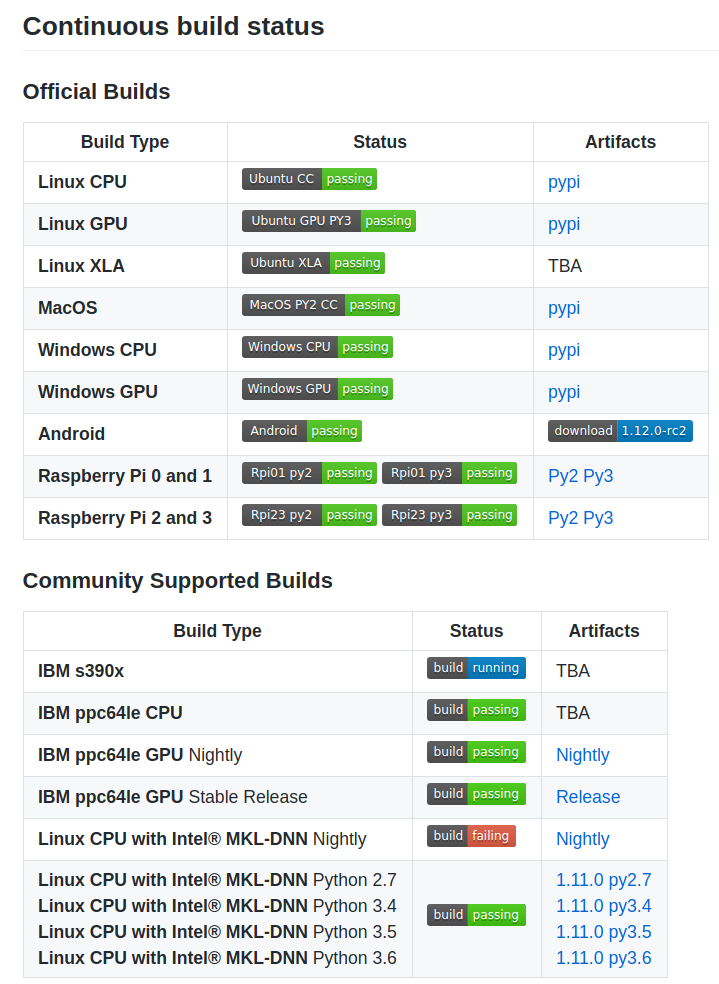
\includegraphics[width=0.7\linewidth]{content/chapter_testing/integration/continuousIntegration}
\end{center}
\end{Frame}